\documentclass[heading.tex]{subfiles} 
\begin{document}

\section{Introduction}

Hyperloop is a conceptual transportation system designed to lower costs and travel times relative to California's current high-speed rail project.
\cite{Musk} Elon Musk and a team of engineers from Tesla Motors and the Space Exploration Technologies Corporation (SpaceX)
proposed the idea in August 2013, as an open design to be vetted and further refined through public contribution.
The concept deviates from existing high-speed rail designs by eliminating the rails, enclosing the passenger pod in a 
tube under a partial vacuum, and suspending the pod on air bearings. Propulsion is handled by a set of linear 
electromagnetic accelerators mounted to the tube, with the entire system being held above ground on concrete 
columns maintaining a straight trajectory.

\begin{figure}[hbtp]
\centering
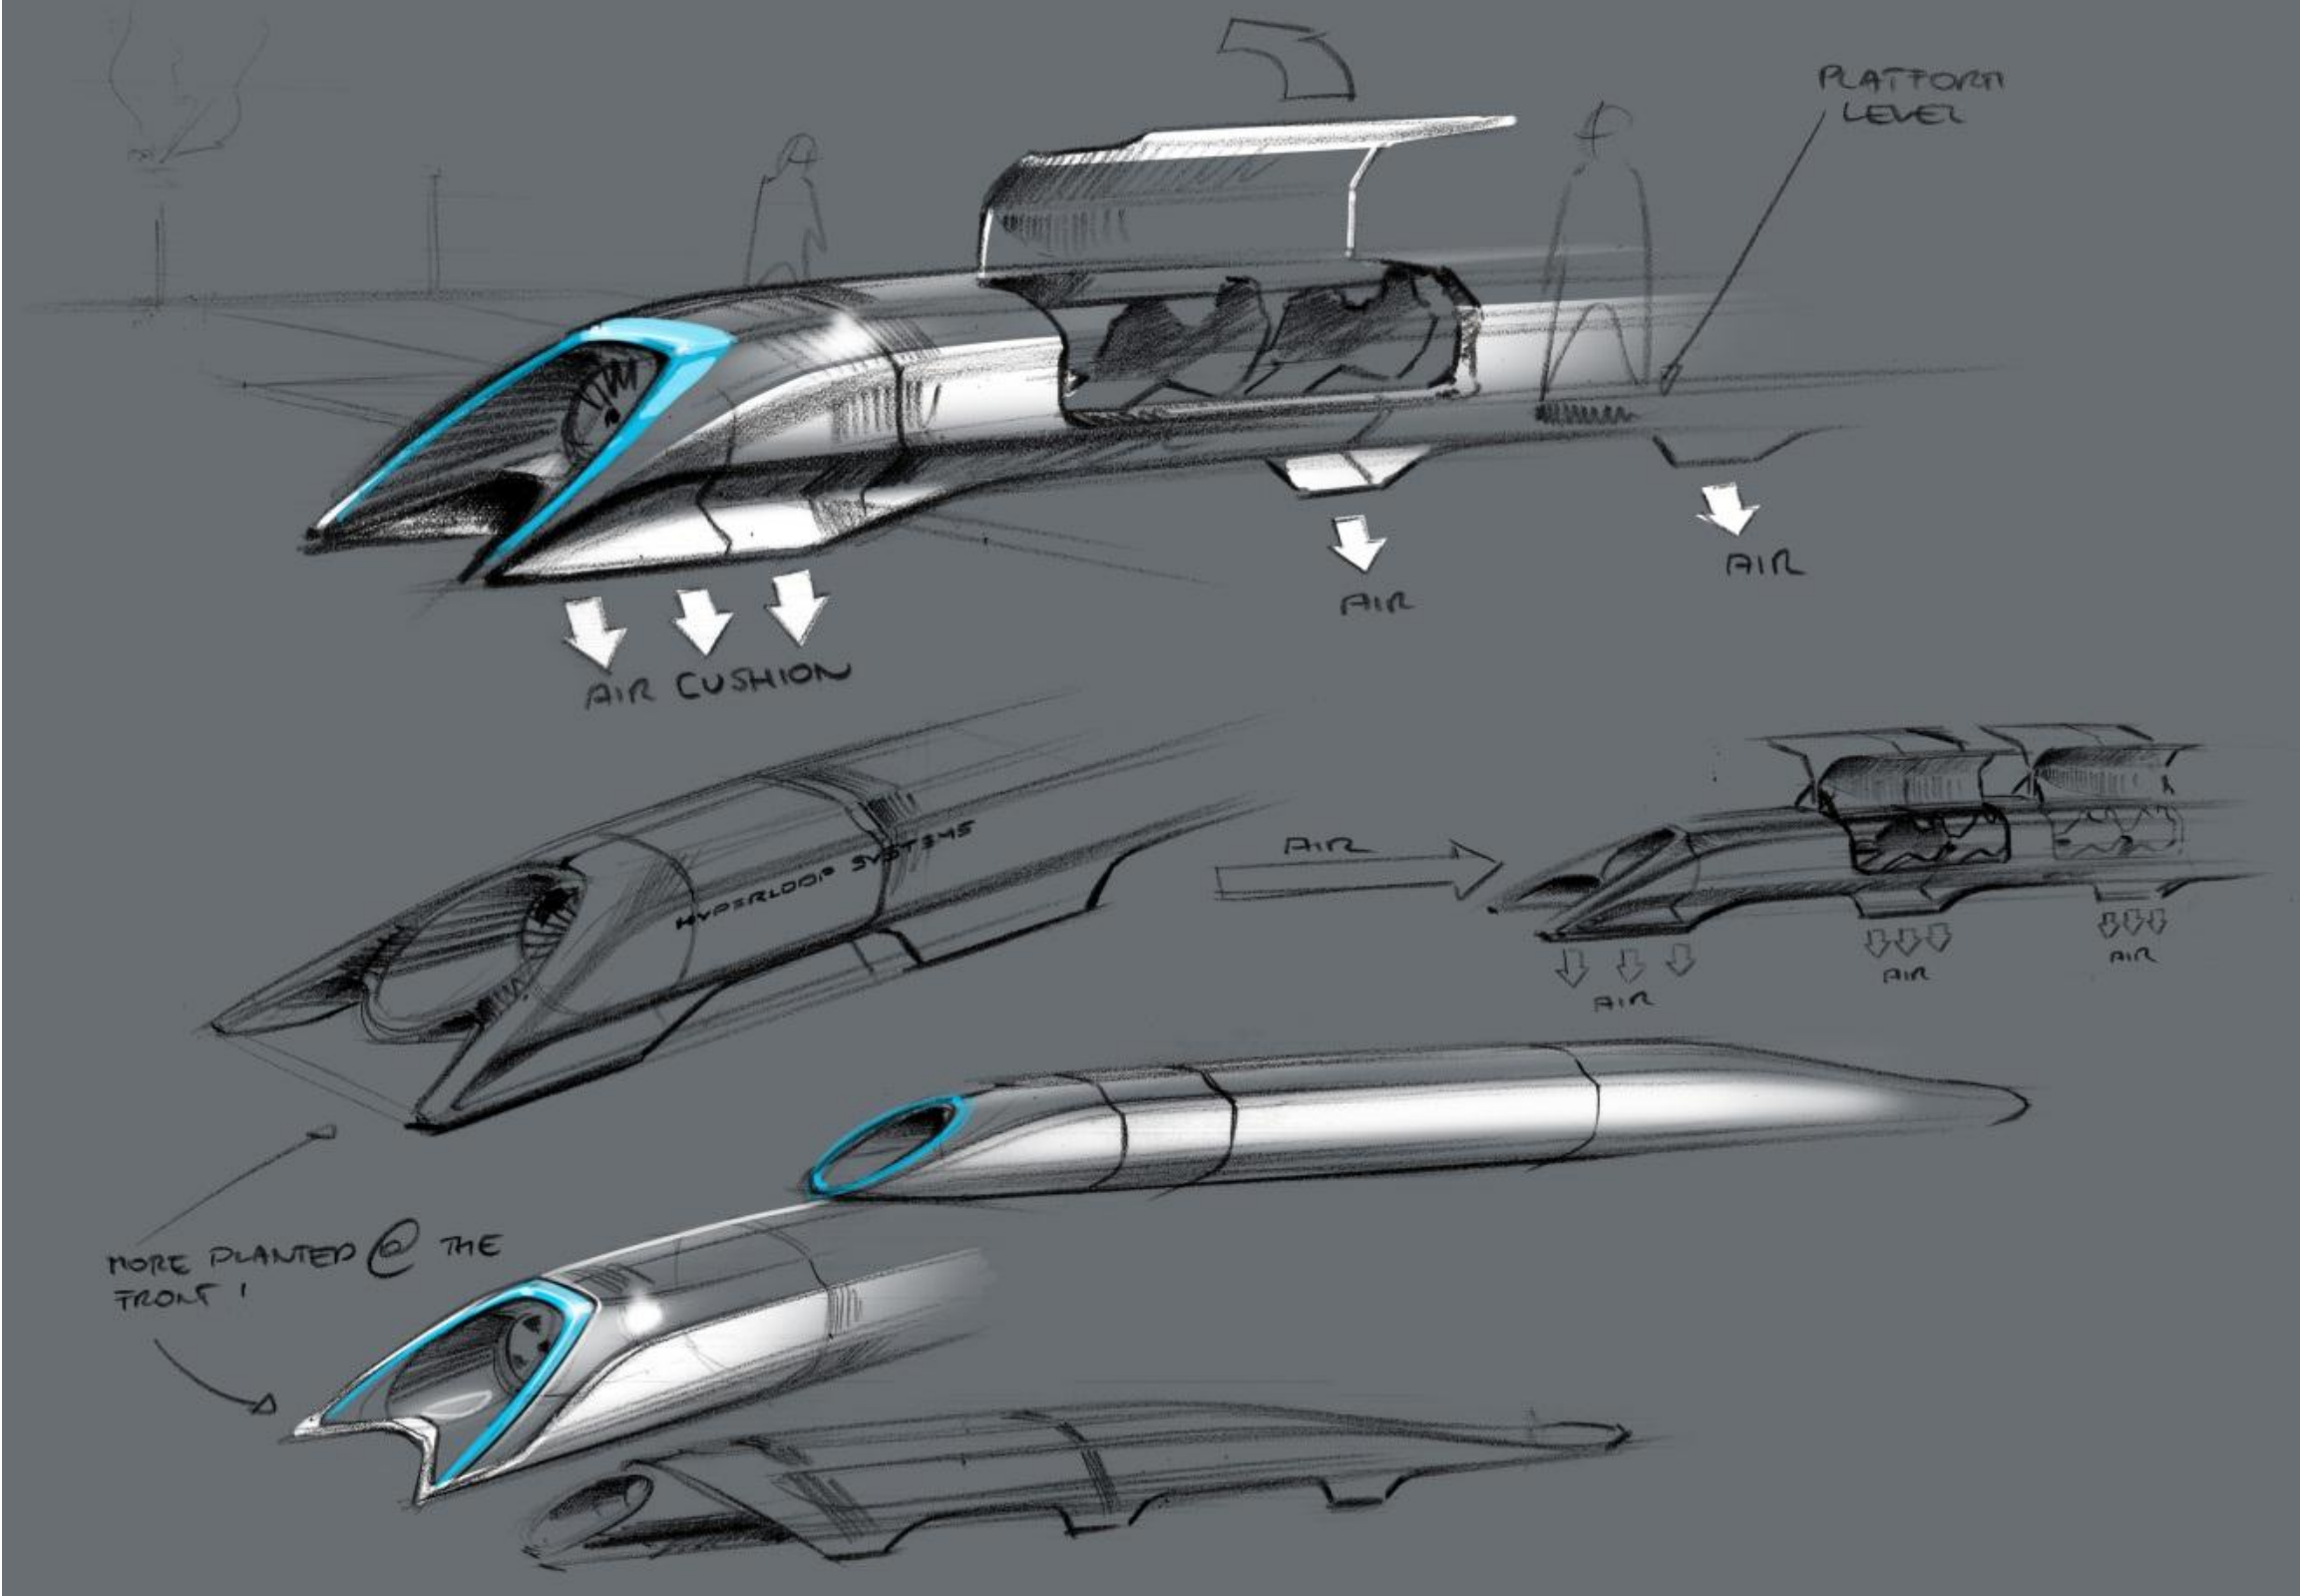
\includegraphics[width=.75\textwidth]{images/hyperloopAlphaSketch.png}
 \caption[Hyperloop Concept Sketch]{Hyperloop-alpha concept sketch of the passenger pod. \cite{Musk}}
\label{f:hyperloopSketch}
\end{figure}

Although Hyperloop is similar to other vacuum tube train (VacTrain) concepts \cite{ET3}, the soft vacuum represents a distinct difference.
It allows the train to run on air-bearings, thus removing the need for a magnetic levitation system used on the other VacTrain designs.
The air bearings require a source of pressurized air, which is provided by an electric compressor system powered by on-board batteries.
Since Hyperloop operates in a partial atmosphere, additional considerations need to be modeled as part of the sizing and thermal analyses. 
The modeling approach applied here is inspired heavily by methods for aircraft sizing and turbine engine cycle analysis. Hyperloop 
operates at transonic Mach numbers in a low pressure environment, so it is straightforward to make the analogy to aircraft. 
The compression subsystem on the passenger pod is similar to the compressors on aircraft turbomachinery. Furthermore, the aerodynamic concerns  
arising from constricted flow through the travel tube are prevalent in the design of inlets for aircraft engines. 

Musk's original Hyperloop proposal included individual high-level analyses of many major subsystems including the pod compression system,
elevated support structure, and propulsion system. While this demonstrated the basic viability of the concept, it did not address
significant interdisciplinary couplings inherent in the Hyperloop system. These couplings introduce certain constraints which limit the 
degrees of freedom available in the design space. The major contribution of this work was to identify the key couplings that constrain the design space
and adapt methods from aircraft design to construct a conceptual design process that accounts for them. The most significant 
interdisciplinary coupling arose between passenger pod size and travel tube size. Aerodynamic concerns make it impossible to vary 
both pod size and tube size independently of each other. An additional, though less severe, coupling arose between the compression system and 
the thermal management system. The interdisciplinary coupling demanded the use of an iterative sizing procedure that balanced 
all the various systems to provide a feasible design for any given set of design variables. The results of this sizing process show that
the Hyperloop concept is feasible, but certain estimates from the original proposal may have been overly optimistic. 

The sizing process is a necessary precursor before ultimately performing a design optimization of 
Hyperloop with the dual objectives of minimizing ticket cost and travel time. Performing this optimization 
was outside the scope of this work and is reserved for future investigation. 
The fully integrated system model was constructed using OpenMDAO, a Python-based framework for 
the design and optimization of highly coupled systems\cite{GrayBenchmarking2013}. The models presented 
in this work represent very basic analyses which rely heavily on simplifying assumptions. A realistic design 
optimization will require more detailed models of the investigated systems and additional analyses for economic models and 
structural models. Adding all of this will result in significant growth in complexity of the Hyperloop model. 
OpenMDAO could provide the means to manage growing model complexity 
in an efficient and flexible manner. Musk's original work was released with the stated goal of jump starting
a crowd sourced design effort. In that spirit all the analyses used in this work have been released under
the Apache V2.0 open source license so that they could potentially serve as a foundation for future work. 
Links to the source code can be found in \cref{app:Github}

The rest of this paper is organized as follows. In section \ref{s:struct} we describe the structure of the Hyperloop 
model. Section \ref{s:sizing} covers the details of the coupling between the primary systems and the impact these have 
on the passenger pod dimensions and performance. Next section \ref{sec:compressor-and-battery}
investigates the battery requirements for the proposed Los Angeles to Sanfrancisco routes considering the effects 
of maximum travel speed. Last, section \ref{s:heatex} investigates the natural thermal equilibrium of the passenger pod and
travel tube to provide a means of sizing the thermal management system. 

% \begin{figure}[hbtp]
% \centering
% 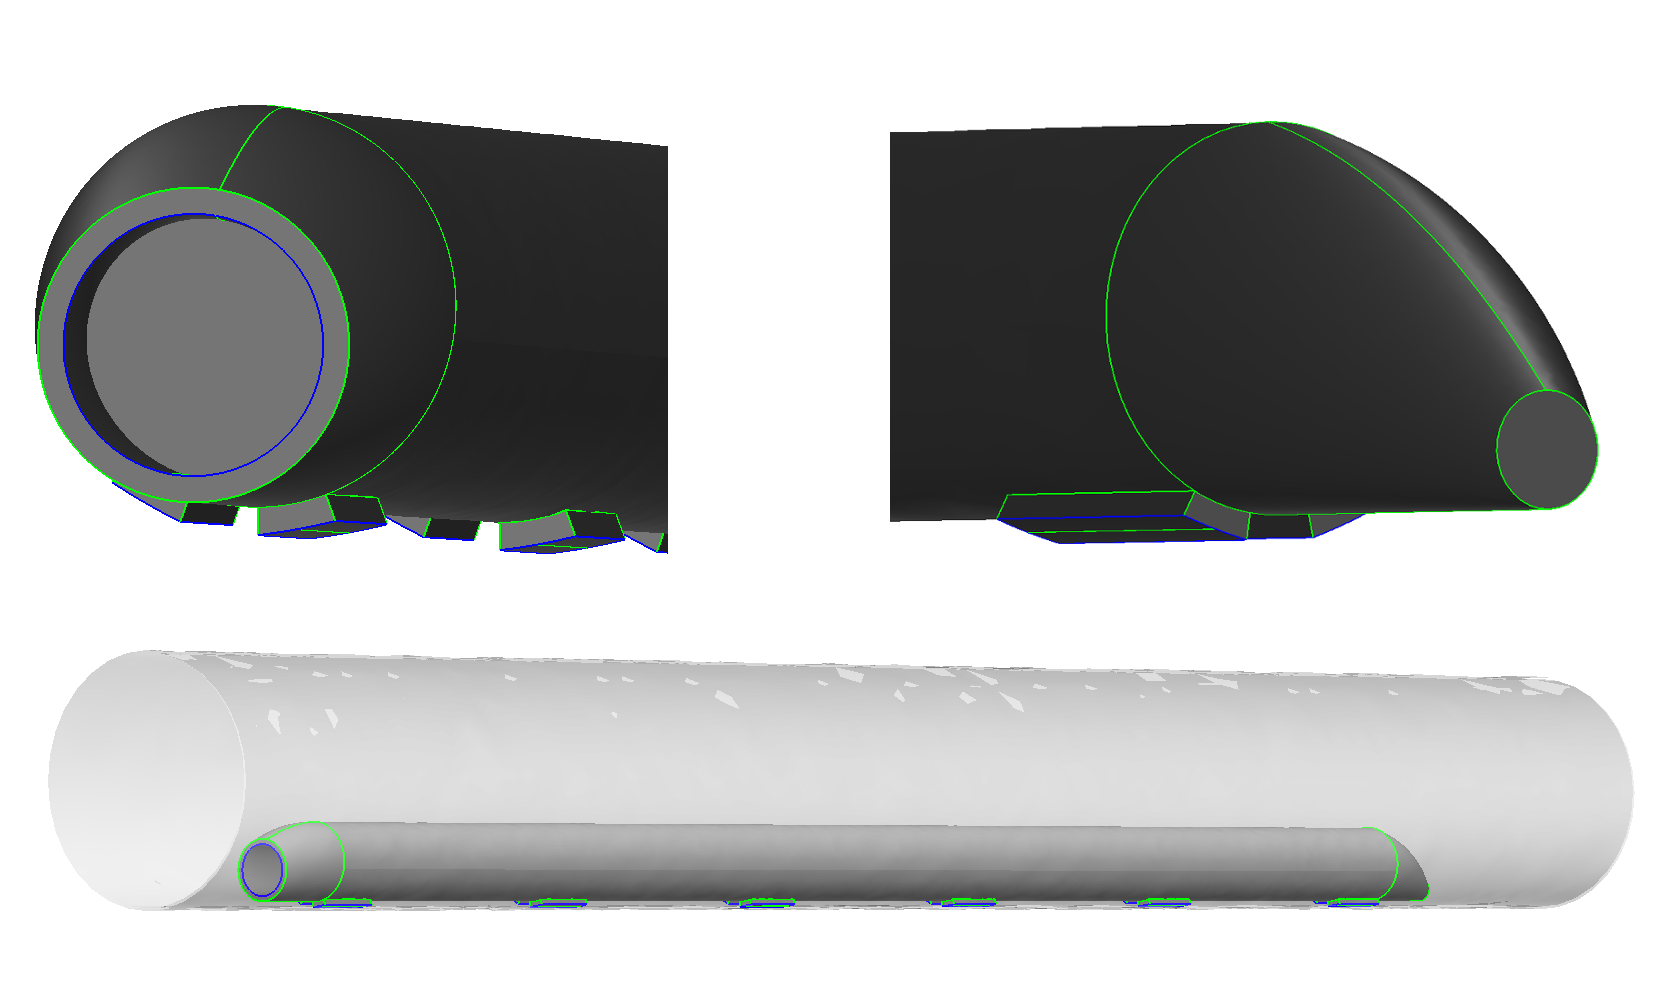
\includegraphics[width=\textwidth]{images/hyperloop_cad.png}
%  \caption[Hyperloop geometry assembled in OpenCSM]{Calculated baseline inlet (left), nozzle (right), and full assembly (bottom) for a pod speed of Mach 0.8. Geometry rendered in OpenCSM, a parametric solid modeling tool.}
% \label{f:hyperloopCAD}
% \end{figure}


\section{Hyperloop Model Overview}
\label{s:struct}
% A large interdependence between the various Hyperloop subsystems stem
% from design variables dictated by the tube and passenger pod systems.
% This coupling, along with other feedback relationships discussed later, require an
% iterative approach to arrive at a physically valid state for the entire system.

The Hyperloop passenger pod was decomposed into five primary analyses that were connected to 
form the conceptual sizing model. 

\begin{enumerate}
  \item Compression System: Performance and power consumption of the compressors.
  \item Mission Analysis: Estimate of travel time and velocity profile.
  \item Pod Geometry: Physical dimensions of the passenger pod.
  \item Tube Flow Limitations: Pod speed limitations based on choked flow restrictions.
  \item Tube Wall Temperature: Equilibrium temperature of the tube.
\end{enumerate}

The relationship between the systems is illustrated in Fig. \ref{f:hyperloopXDSM}. Feed forward connections 
are represented as the blue arrows in the upper right side of the diagram. For example, the \textit{Compressor Cycle} 
passes data to the \textit{Mission Analysis}, \textit{Pod Geometry}, and \textit{Tube Temperature} analyses. In the lower left 
side of the diagram red arrows represent feed back connections which establish coupling between different 
analyses. The top left block of Fig. \ref{f:podXDSM} shows design variables that affect 
different systems. Table \ref{tab:desvars} summarizes the baseline values as well as ranges selected 
to provide a reasonably large design space. Notably, both Pod radius and travel tube radius are missing 
from the list of variables in Table \ref{tab:desvars}. These variables could not be freely varied. Instead, the assumption of a fixed area for a passenger compartment was made which, combined with the couplings shown in Fig. \ref{f:hyperloopXDSM}, removed these variables as design inputs. This issue will be discussed in much greater detail in Section~\ref{s:sizing}.

\begin{table}
    \centering
    \caption{Hyperloop passenger pod design variables}
    \label{tab:desvars}
    \begin{tabular}{l  c  c  c} 
        \hline
        Variable & Baseline Value & Min. & Max. \\ \hline 
        Max. Pod Mach & .9 & .3 & 1.0 \\ 
        Pod Bypass Mach & .95 & .5 & .99 \\
        Compressor 1 Inlet Mach & .6 & .5 & .8 \\ 
        Compressor 1 Pressure Ratio & 12.47 & 10 & 20 \\ 
        Tube Static Pressure (Pa) & 99 & 50 & 500 \\ \hline
    \end{tabular}
\end{table}

\begin{figure}[hbtp]
\centering
\includegraphics[width=\textwidth]{images/TopAssembly.png}
\caption{Workflow and dependencies between the major Hyperloop subsystems.}
\label{f:hyperloopXDSM}
\end{figure}

The compression system and pod geometry analyses were each further subdivided into a number of subsystems. For this work the pod geometry 
system was primarily responsible for computing important areas throughout the passenger pod. Figure \ref{f:podXDSM} shows the 
pod geometry breakdown into 5 subsystems. Most of these calculations were based on simple geometric relationships. The 
modeling was broken down to enhance modularity so that future work could replace these simple analyses with more advanced ones.
The pod geometry system is the place to include structural and weight estimation models for the passenger pod in future work,
though these analyses were outside the scope of this work. 

\begin{figure}[hbtp]
\centering
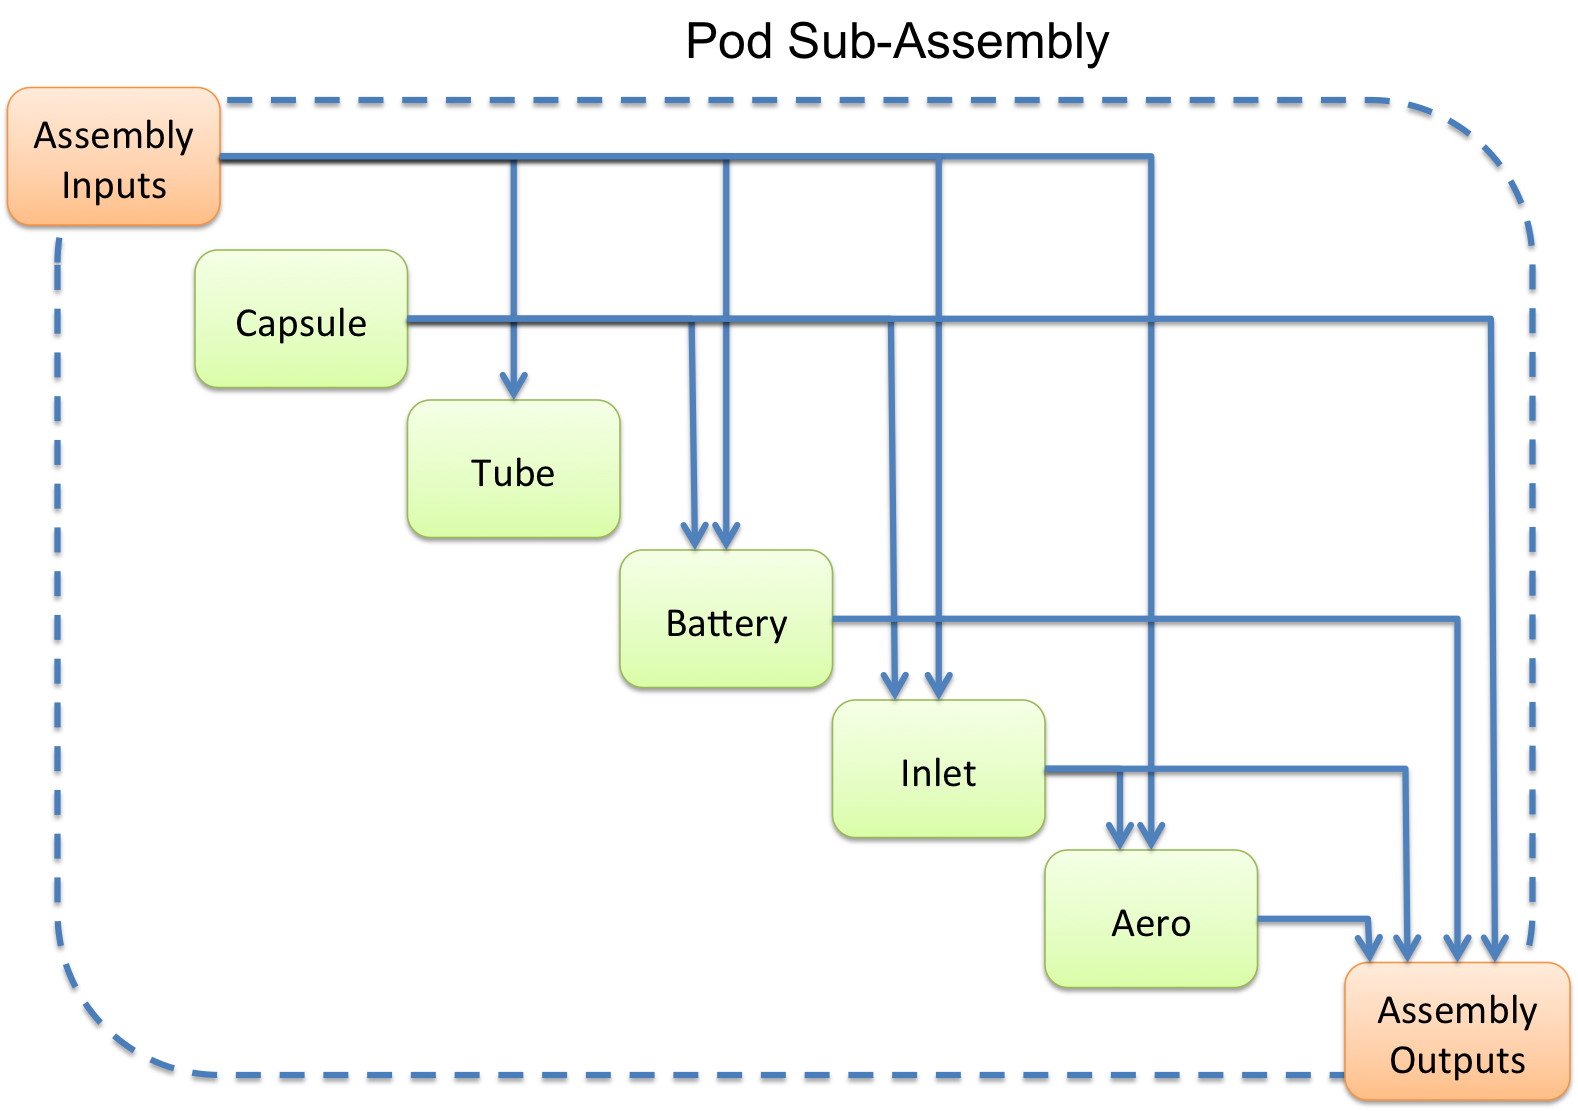
\includegraphics[width=\textwidth]{images/podAssembly.png}
\caption{Expanded \texttt{pod} assembly XDSM}
\label{f:podXDSM}
\end{figure}

The compressor cycle performed calculations related to the thermodynamic processes of compressing, cooling, and exhausting air. 
The modeling approach for the compressor cycle was heavily influenced by techniques developed in the Numerical Propulsion System Simulation (NPSS) code. 
NPSS was created as a joint effort between United States engine manufacturers and NASA Glenn Research Center for the purpose of 
simulating and analyzing turbomachinery cycles for aircraft applications\cite{Lytle}. NPSS employs a highly modular model construction
where cycles get broken down into individual thermodynamic processes and then connected together. This modularity was adopted for pyCycle, 
the cycle modeling tool used in this work. PyCycle was used to predict the mass flow and power consumption of the entire compression system. 
In the original hyperloop proposal, the air bearings were specified to work with a static pressure of 11 kPa. The compression system is modeled as two separate compressors, with the first compressing the air to bypass the pod internal structure and passenger compartment and the second providing additional pressure to reach the required 11 kPa. The required pressure ratio for the second stage
is a function of the maximum pod Mach number and the first stage compressor pressure ratio. In Fig. \ref{f:compressorXDSM} this relationship 
shows up as a feedback connection between the performance and the compressor 2 subsystems. 

\begin{figure}[H]
\centering
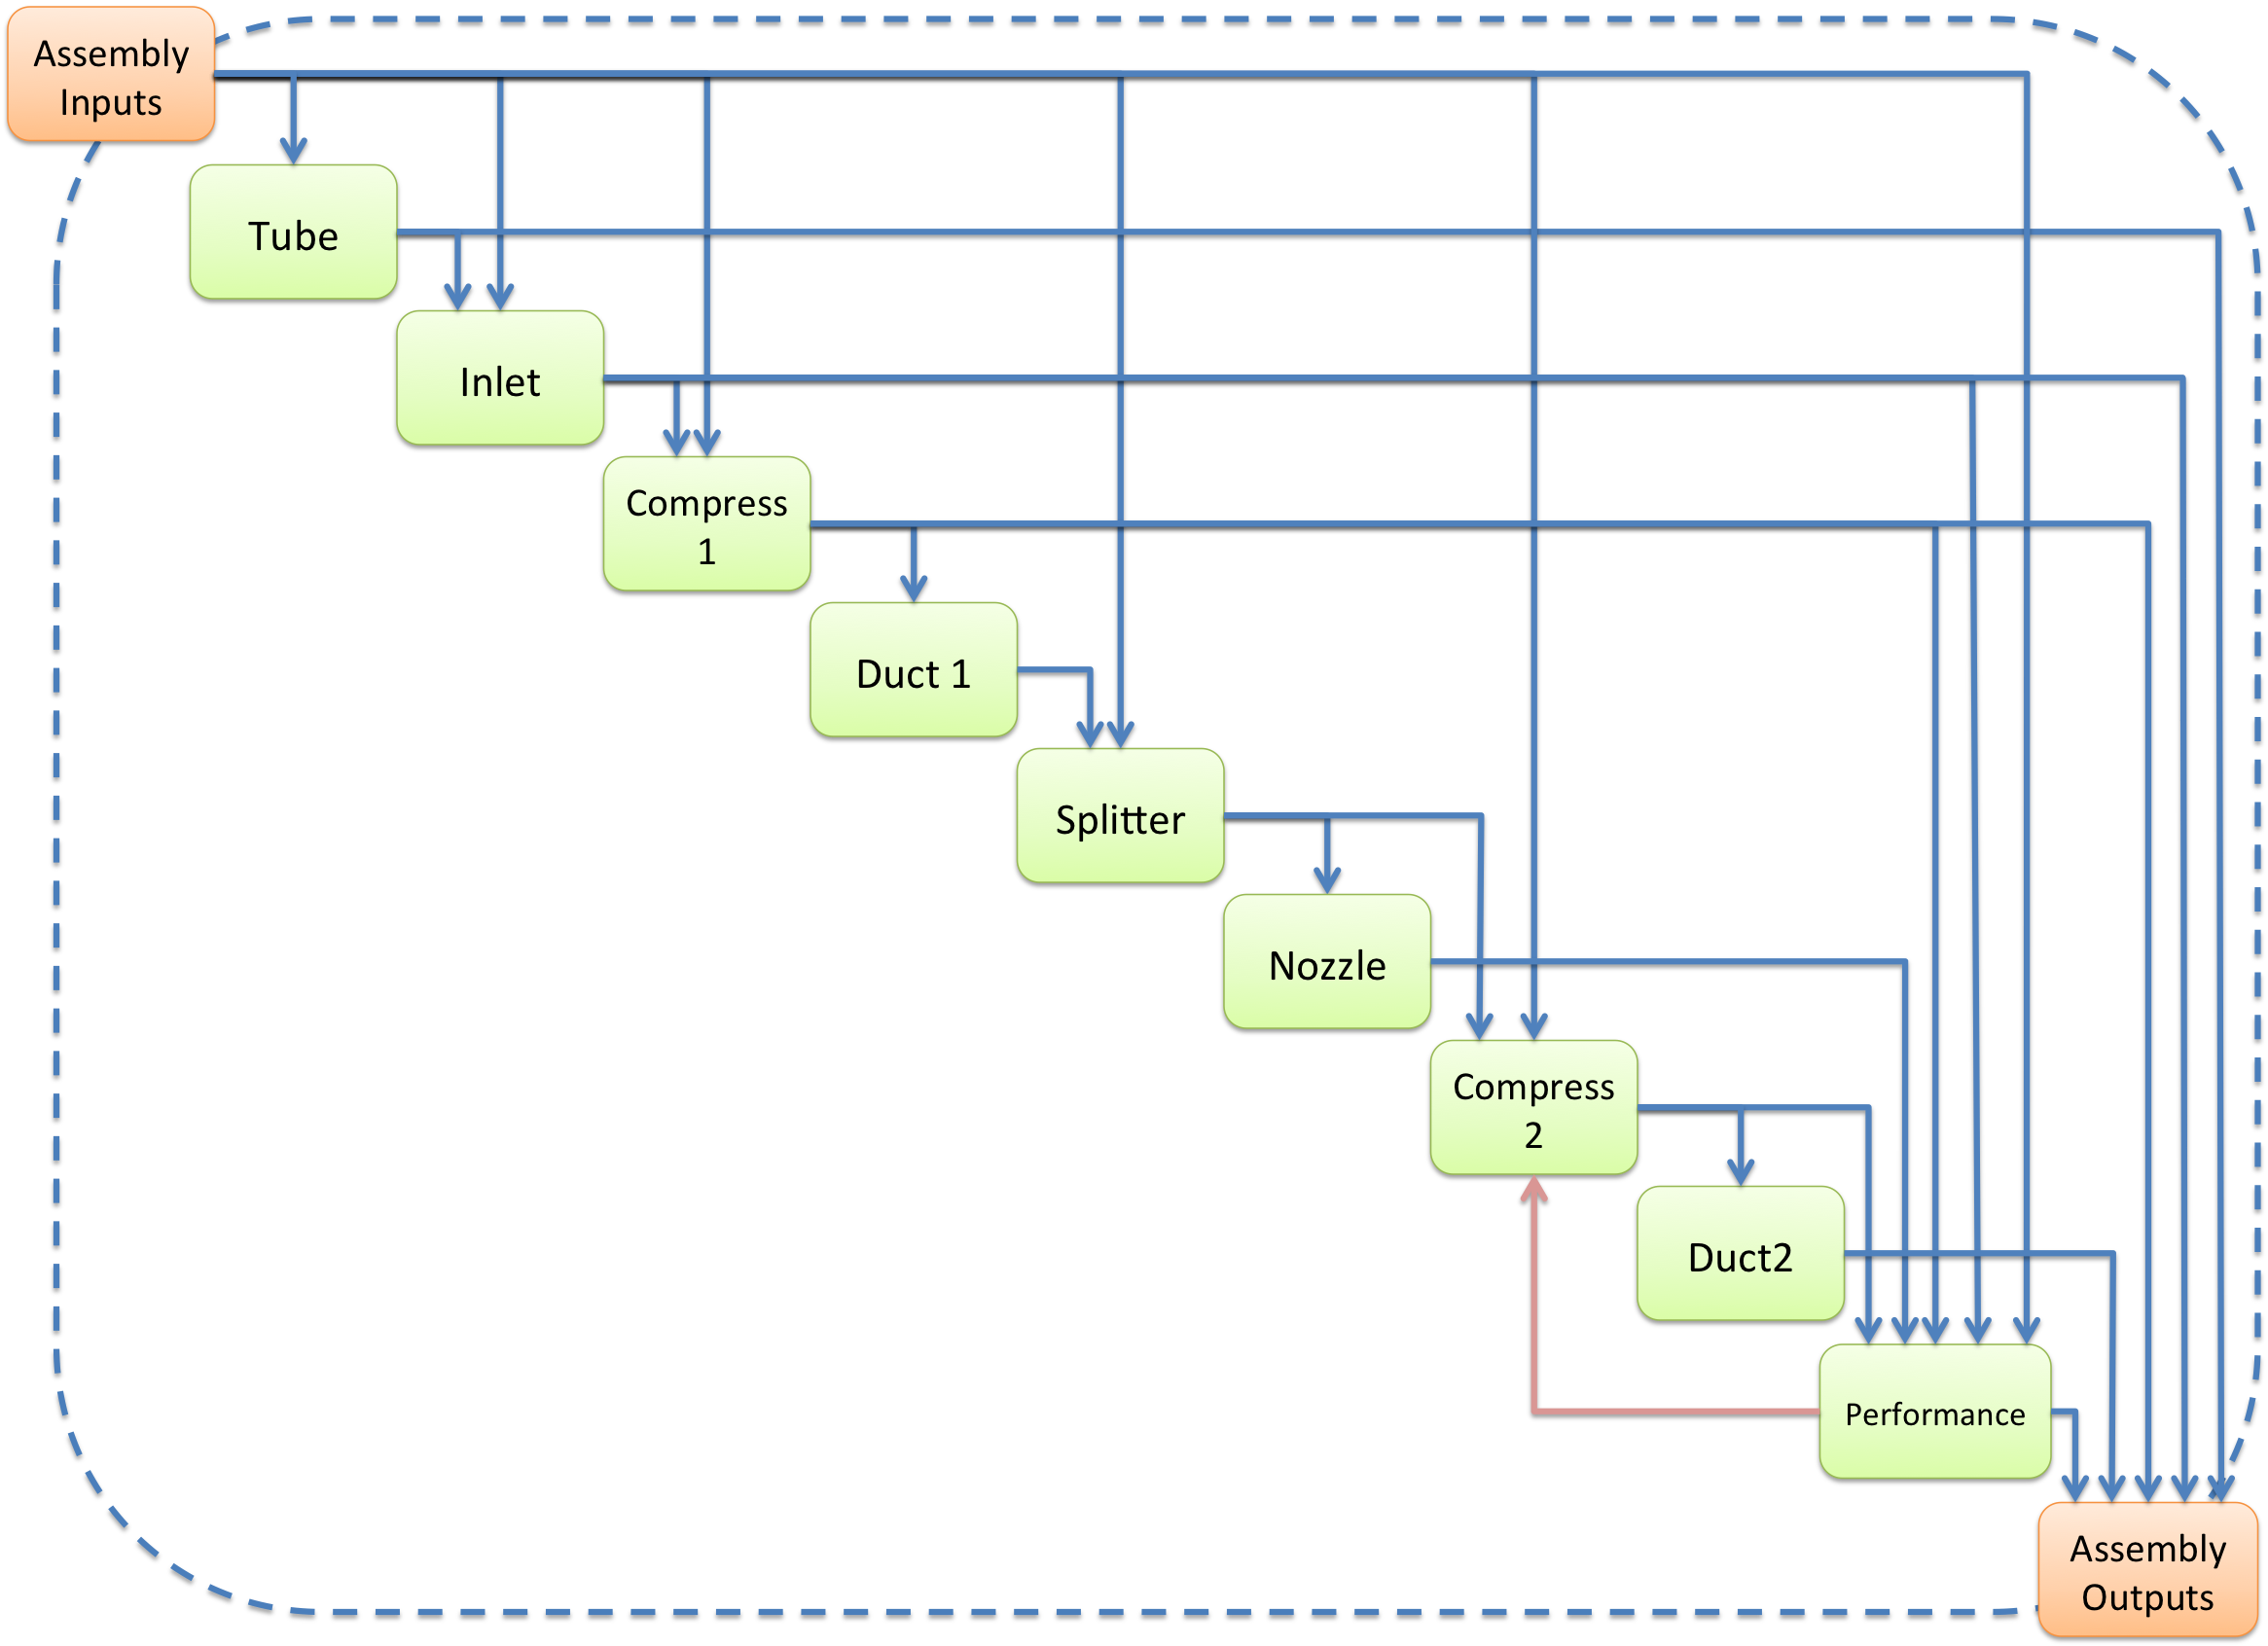
\includegraphics[width=\textwidth]{images/compAssembly.png}
\caption{Expanded \texttt{compress} assembly XDSM}
\label{f:compressorXDSM}
\end{figure}


\section{Pod and Tube Sizing}
\label{s:sizing}

In the original Hyperloop proposal, the size of the passenger pod and the travel tube were treated as design variables, 
free to vary within reasonable ranges independent of each other. Two different configurations were proposed: a smaller 
pod for passengers and a larger pod for cargo. The two configurations, with overall dimensions summarized 
in Table \ref{t:hyperbase}, had a slightly different ratios of tube area to pod area. 

\begin{table}
  \centering
  \caption{Dimensions of the passenger and cargo hyperloop designs from the original proposal. }
  \label{t:hyperbase}
  \begin{tabular}{l c c}
    \hline
                                  &  Passenger       & Passenger + Cargo \\ \hline
    $r_{tube}$ ($m$)              &        1.11      &     1.65  \\
    $A_{tube}$  ($m^2$)           &        3.87      &     8.55  \\
    $A_{pod}$ ($m^2$)             &        1.4       &     4.0   \\ 
    $A_{bypass}$ ($m^2$)          &        2.47      &     4.55  \\ 
    $\frac{A_{bypass}}{A_{tube}}$ &        .64       &     .53   \\
    Max Mach                      &        .95       &     .95   \\
    \hline
  \end{tabular}
\end{table}

\begin{figure}[hbtp]
\centering
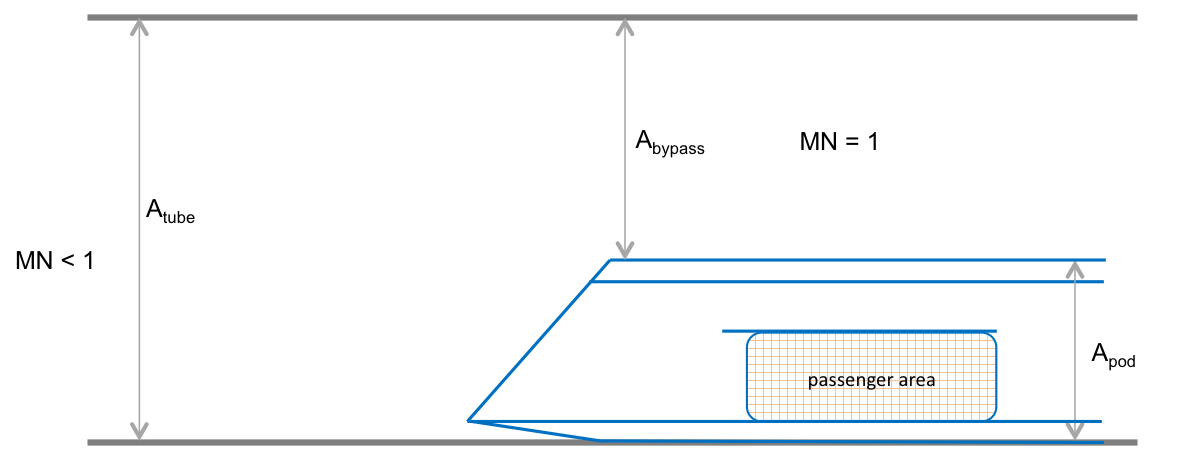
\includegraphics[width=.85\textwidth]{images/podA}
\caption{Longitudinal view of a passenger pod with no inlet and no compression system.}
\label{f:ClosedPod}
\end{figure}

Smaller tube sizes are preferable because they provide lower construction costs. However, it can be shown that 
the tube size is coupled to the speed of the air as it passes around the pod of a given size. 
To understand this coupling consider the following simplified situation: assume that a sealed pod
is traveling through a frictionless tube from right to left, at some $M_{pod}$ less than 1, through a stationary mass of air. 
Figure \ref{f:ClosedPod} depicts this situation. For the purposes of analysis it is more convenient to consider the opposite perspective, 
where the pod is stationary and the air is moving from left to right with some relative Mach number, $M_{pod}$. 
As the air moves around the pod, it must fit into the smaller space available to it, $A_{bypass}$, which causes the air 
to accelerate to some higher Mach number, $M_{bypass}$. From isentropic flow equations, there is a relationship between 
$M_{pod}$ and $M_{bypass}$ that defines $\frac{A_{bypass}}{A_{tube}}$.

\nomenclature{\gamma}{Heat Capacity Ratio}
\nomenclature{MN}{Mach Number}
\begin{equation}
\frac{A_{bypass}}{A_{tube}} = \frac{M_{pod}}{M_{bypass}}
\left(\frac{1+ \frac{\gamma-1}{2} M_{pod\ \ \ }^2}
{1+ \frac{\gamma-1}{2} M_{bypass}^2}\right)^{\frac{\gamma+1}{2\left(1-\gamma\right)}}
\label{e:a-over-astar}
\end{equation}
%\left(\frac{\gamma+1}{2}\right)^{-\frac{\gamma+1}{2\left(\gamma-1\right)}}\frac{\left(1+\frac{\gamma-1}{2}M_{pod}^{2}\right)^{\frac{\gamma+1}{2\left(\gamma-1\right)}}}{M_{pod}}

\begin{figure}[!htb]
  \centering
  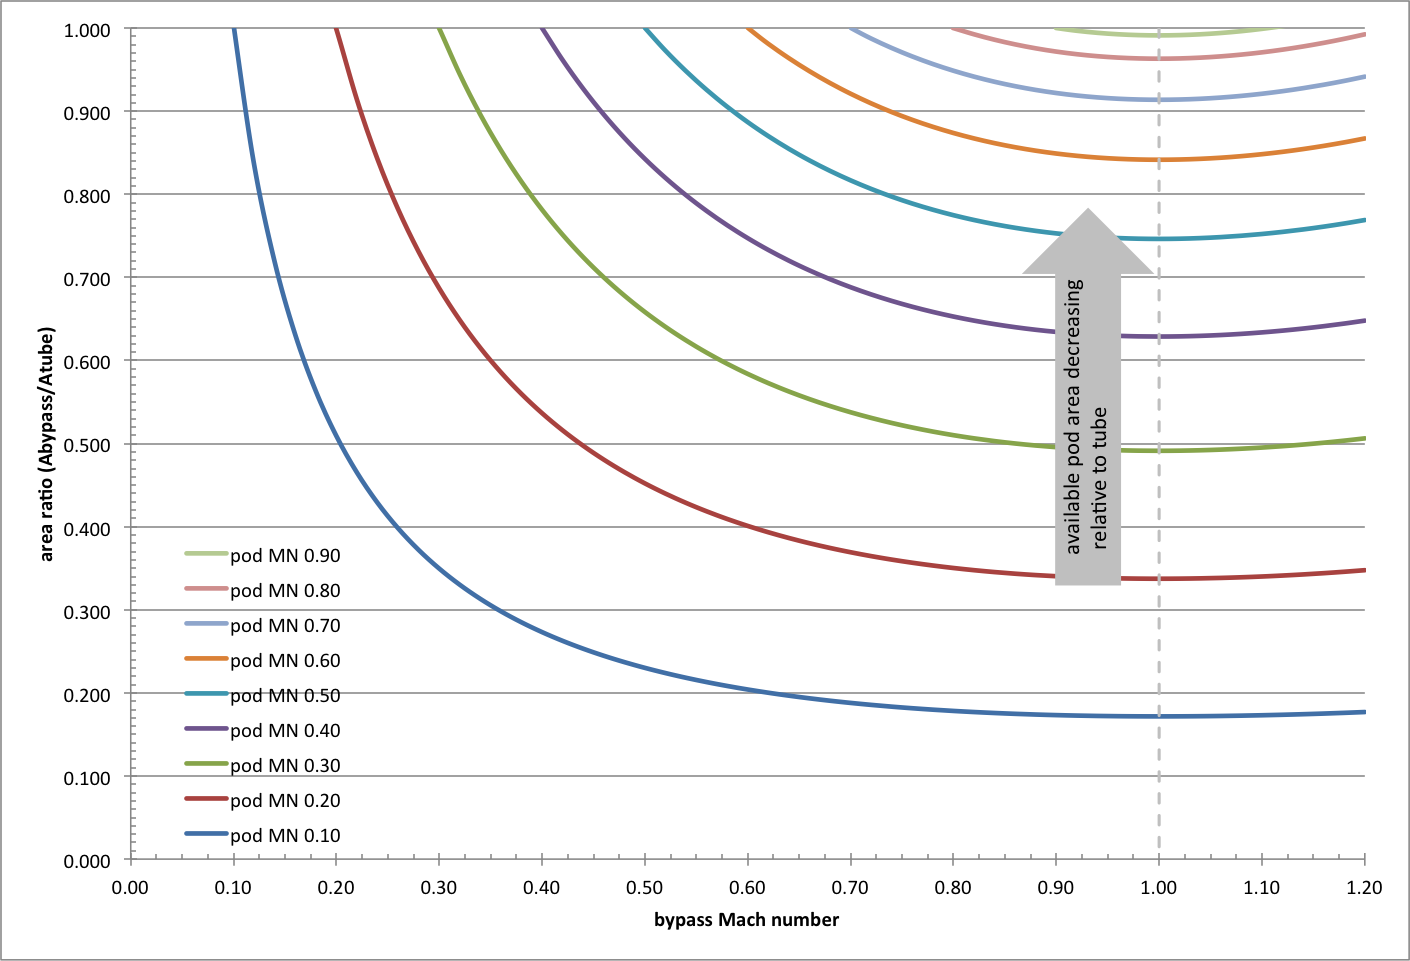
\includegraphics[width=.9\textwidth]{images/choked-flow}
  \caption{The area ratio required reaches a minimum value at $M_{bypass}=1$ for all values of $M_{pod}$}
  \label{f:choked-flow}
\end{figure}

Figure \ref{f:choked-flow} depicts an investigation of Eq.~(\ref{e:a-over-astar}) over a range of values for $M_{pod}$ and $M_{bypass}$. 
For all values of $M_{pod}$, the minimum required $\frac{A_{bypass}}{A_{tube}}$ occurs exactly at $M_{bypass}=1$. In other words, 
$M_{bypass}=1$ will always give the smallest possible $A_{bypass}$ (and hence $A_{tube}$) for a given 
$M_{pod}$ and $A_{pod}$. Thus $A_{tube}$ can not be treated as an independent design variable. If you forced $A_{tube}$ to be
smaller than this minimum value, then not all the relative mass flow could pass freely around the pod. This excess 
flow would accumulate in the left of Fig. \ref{f:ClosedPod}), with the pod acting like a piston pressurizing the 
air in front of it. 

Furthermore, Fig. \ref{f:choked-flow} also shows that the required $\frac{A_{bypass}}{A_{tube}}$ 
increases with increasing $M_{pod}$. So the faster the pod travels, the larger $A_bypass$ 
must become to accommodate the relative mass flow around it. For $M_{pod}$ equal to 1, $\frac{A_{bypass}}{A_{tube}}$ must 
equal 1 as well, forcing $A_{pod}$ to be 0. So it is physically impossible for a closed pod to travel through a 
tube with $M_{pod}$ at the speed of sound. Note that the Table \ref{t:hyperbase} gives area ratios around .6, 
which would then yield a maximum $M_{pod}$ of about .35. 

\begin{figure}[hbtp]
\centering
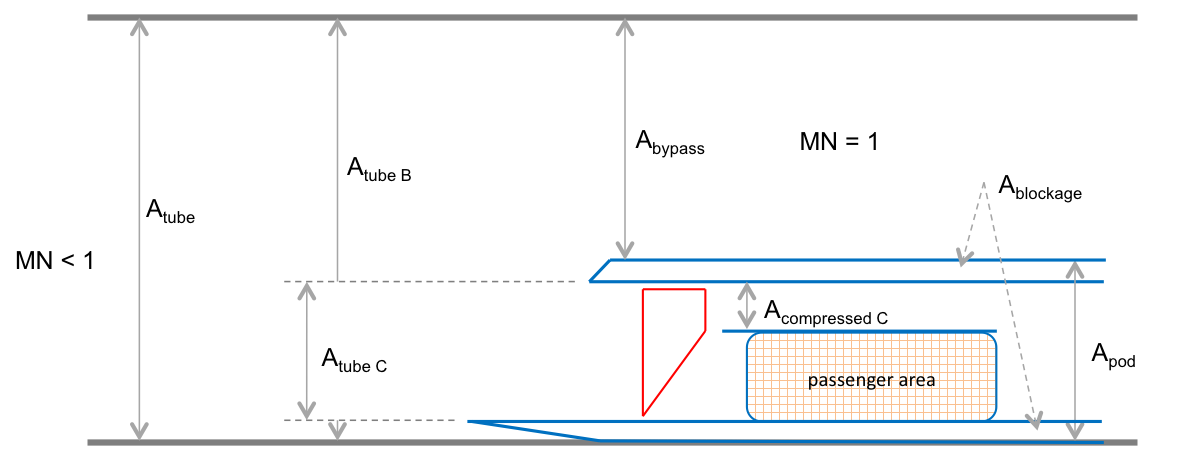
\includegraphics[width=.85\textwidth]{images/podB}
\caption{Longitudinal view of a hollow passenger pod that lets mass flow pass through it.}
\label{f:hollowPod}
\end{figure}

To get around this limitation Hyperloop allows some mass flow to pass through the pod itself, thereby increasing
the maximum achievable speed. This effectively splits the relative mass flow in $A_{tube}$ into two streams, 
$A_{tube\ B}$ and  $A_{tube\ C}$, as shown in Fig. \ref{f:hollowPod}. If we neglect the small thickness of the walls of
the passenger pod itself, and assume that $A_{tube\ C}$ is equal to the $A_{pod}$, then it follows that $A_{tube\ B}$ 
will be equal to $A_{bypass}$. Without any area contraction the flow in the bypass would not accelerate, staying 
at $M_{pod}$. The challenge is that the pod can not be perfectly hollow. It must provide some space for the passengers
to sit in, causing some blockage in the flow. This problem can be handled by adding a compression system to the 
pod that will force the air into a smaller area $A_{compressed\ C}$, to move around the passengers. This would 
seem to solve all of the challenges associated with high travel speeds inside a tube discussed above and decouple 
$\frac{A_{bypass}}{A_{tube}}$ and ${M_pod}$.


\begin{figure}[hbtp]
\centering
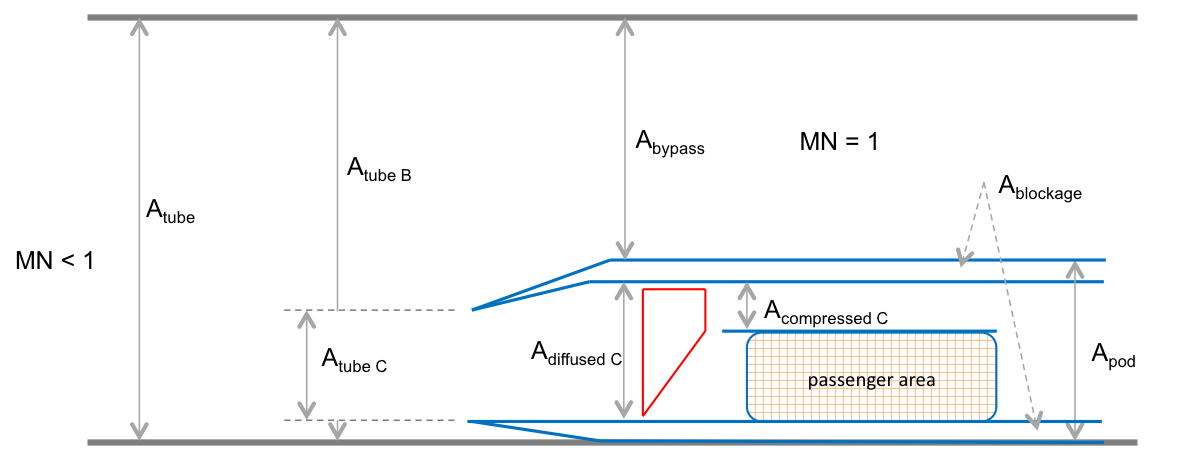
\includegraphics[width=0.85\textwidth]{images/podC.png}
\caption{Longitudinal view of a hollow passenger pod with a necessary diffuser to restrict the Mach number of the flow into the compressor.}
\label{f:OpenPod}
\end{figure}

In order to achieve reasonable efficiency from the compression system, the Mach number of the flow at the compressor face
must be limited to less than about .65. So for $M_{pod}$ greater than .65, a diffuser must be added to the Hyperloop 
which will slow the air down before it enters the compressor. As depicted in Fig. \ref{f:OpenPod}, diffusing the flow 
requires expanding it; $A_{diffuser}$ must be greater than $A_{compressor}$. Unfortunately this means that
$A_{bypass}$ must be smaller than $A_{tube\ B}$, and some acceleration of the flow through the 
bypass will occur. Once again, $\frac{A_{bypass}}{A_{tube}}$ becomes coupled to $M_{pod}$, although thanks to the compression 
system this is now much less restrictive than if the pod was sealed. 

Figure \ref{f:machRAD} shows the increase in pod Mach number achievable for the hollow pod compared to the closed pod. For a nominal tube diameter of ?m, the maximum pod Mach increases from x to y. This increase is strongly dependent on the amount of "blockage" assumed and slightly dependent on the compressor face Mach number. Changing the compressor face Mach number by +-0.05 changes the maximum pod Mach number by roughly +-0.01.
A final note: all of these results are unaffected by the tube pressure. But Ps affects massflow and power discussed next.


\nomenclature{c1MN}{Mach number at the front face of the first compressor}
\begin{figure}[H]
\centering
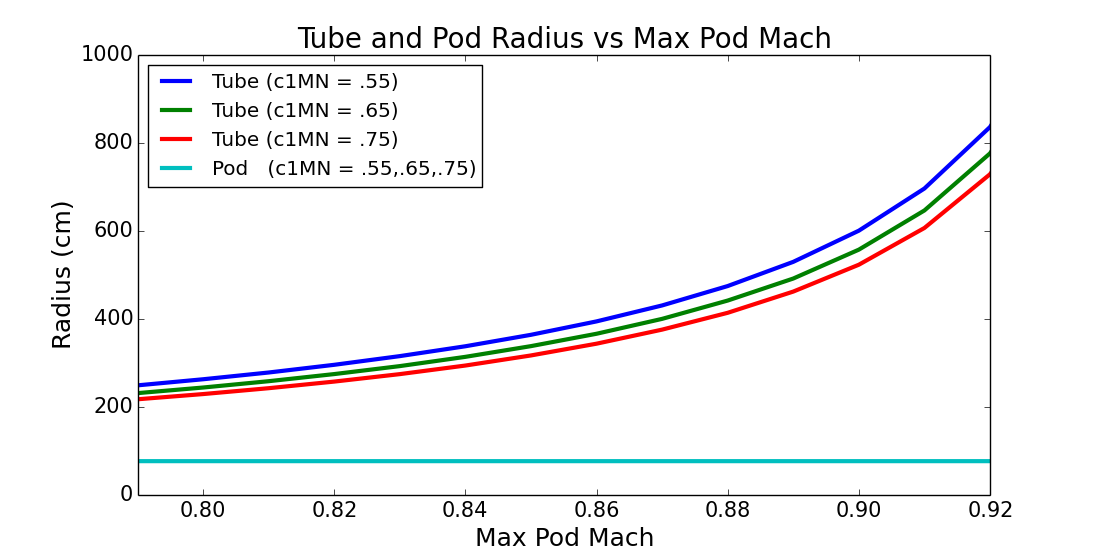
\includegraphics[width=\textwidth]{images/mach_vs_rad4.png}
\caption[Tube and Pod Radius vs Mach]{Exponential relationship between pod speed and required tube radius, for three diffused mach numbers.
Converged pod radius also show underneath. }
\label{f:machRAD}
\end{figure}


\section{Compressor Power and Battery Sizing}
\label{sec:compressor-and-battery}

The on-board compression system serves dual purposes.
It provides a means of increasing the maximum pod speed over a closed pod, and also supplies pressurized air to the air bearing system.
This second function requires a minimum airflow to provide the pressure force necessary to support the vehicle mass.
A thermodynamic analysis of the compressor system is also necessary to
estimate on-board power requirements and overall heat rise of each pod.
The compression cycle is comprised of an inlet, two compressors, a nozzle, and multiple ducts leading to air bearings.
The design deviates from the original proposal by removing two heat exchangers for reasons explained in the following section.
The system, shown in Fig. \ref{f:comp} is modeled as a one-dimensional cycle,
representing components as thermodynamic processes that are subsequently chained together.
Each component is responsible for calculating gas properties across its boundaries
and appropriately enforcing conservation equations across the entire system.

\begin{figure}[hbtp]
\centering
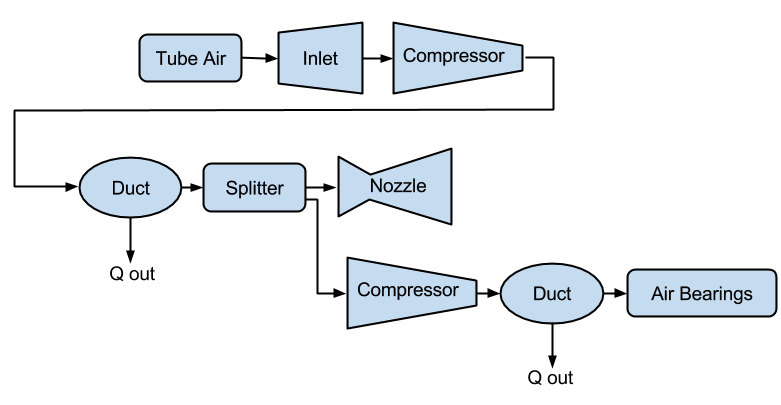
\includegraphics[width=0.9\textwidth]{images/compressor_schematic.png}
\caption{Schematic of the Hyperloop compression system, showing flow connections between components.}
\label{f:comp}
\end{figure}


The simulation uses PyCycle, an open-source cycle analysis tool that employs Cantera [ref] for thermodynamic calculations. The design of PyCycle was heavily influenced by NPSS;
further information on these tools can be found in the appendix and online documentation. \cite{goodwin2009cantera}

The model predicts the instantaneous power consumption of the compressors, temperature and pressure rises,
and upstream conditions necessary to supply sufficient airflow to the bearings.
These power requirements are a function of the chosen cycle and are both affected by
and contribute to the thermal conditions, creating the feedback loop “C” in Fig. \ref{f:hyperloopXDSM}.
Combined with the mission profile described below, these requirements impact battery sizing.

\begin{figure}[hbtp]
\centering
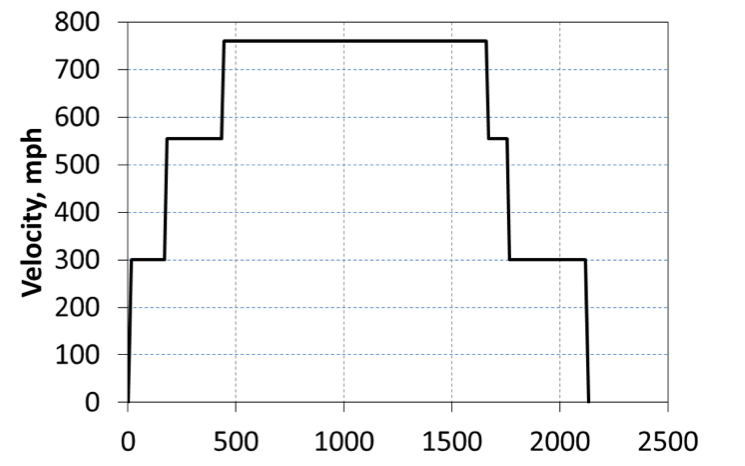
\includegraphics[width=0.7\textwidth]{images/velocity_profile.png}
\caption{Velocity profile described in the original proposal}
\label{f:velocity}
\end{figure}

Using the notional velocity profile described in the original proposal, and shown in Fig. \ref{f:velocity},
a speed factor can be estimated by normalizing the profile then scaling it based on the maximum
attainable velocity calculated in the previously discussed subsystems.
From the resulting speed factor, or ratio of average speed to maximum speed,
a crude estimate of total travel time can be deduced based on total tube length.
Multiplying this time by the average compressor power consumption and a 30\% safety margin results in an overall battery storage requirement.

\begin{figure}[hbtp]
\centering
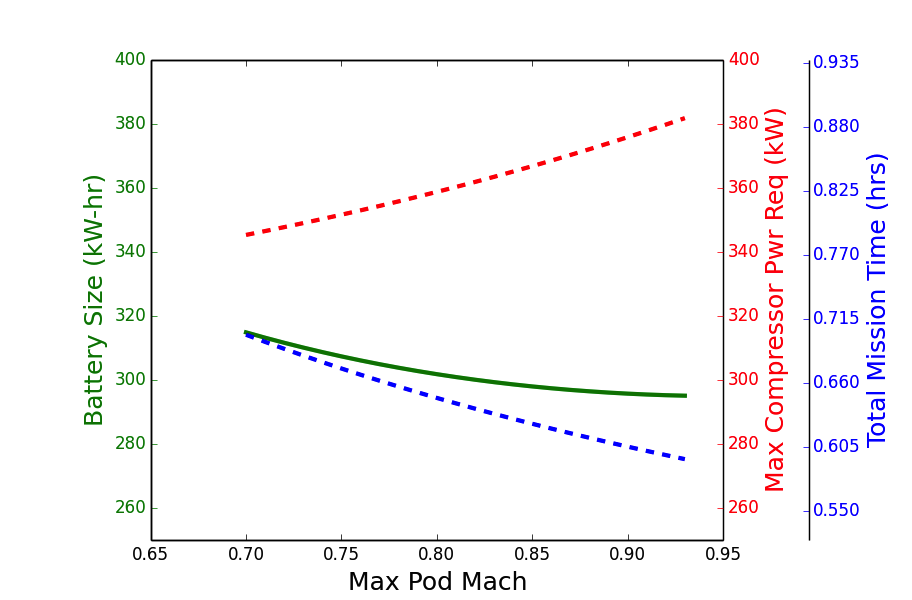
\includegraphics[width=\textwidth]{images/battery_plot.png}
\caption[Battery requirements as a function of pod speed]{Battery requirements as a function of pod speed. Note: the y-axis begins at 340kW-hr.}
\label{f:battery}
\end{figure}

The necessary on-board battery size was found to be inversely related to the max pod speed, as shown in Fig. \ref{f:battery}.
This indicates that compressor power requirements are less sensitive to increased speeds than total trip time.
Although traveling at higher speeds draws more energy, the system is operated for a shorter period of time.
This sensitivity is highly dependent on the velocity profile.
Therefore, reducing time spent at max speed could result in a positive correlation between battery size and pod speed.
It should also be noted that the Y-axis of Fig. \ref{f:battery} begins at 340kW to emphasize the downward trend.
The overall reduction in battery size is on the order of 25\%, if speed is increased from Mach 0.7 to Mach 0.9.
Additional mission analysis details can be found in \cref{app:route} and work done by Mathworks \cite{Rouleau}.
These estimates are in agreement with Musk’s work, and equate to roughly 3 to 5 battery packs from a Tesla Model-S.
However, the estimates are still optimistic since no work has been done to estimate battery cooling requirements,
and based on the assertion that the compression cycle does not need to be cooled.
The system-level thermal interactions and heat exchangers are analyzed next.

\section{Heat Exchanger and Tube Thermal Analysis}
\label{s:heatex}
As each pod passes through the tube, it adds energy to the air in the form of heat.
Following the proposed frequency of launching a pod every six minutes,
the continuous operating cycle could potentially heat the overall tube to excessive temperatures.
To combat this effect, the original proposal recommends a heat exchanger that would be integrated into the compression system.
These intercoolers would use water stored in on-board tanks to cool the air and assist secondary compression.
The resulting steam could then be stored in a tank and offloaded once the pod reached its destination.
However, initial calculations show that using water for cooling is not an ideal design for two reasons:

1) The flow rate of water needed to remove the heat added by the compressors is very large, and the sheer volume constraints of storing
the resulting steam would outweigh the benefits.

2) The heat addition from each pod compressor cycle is fairly low relative to other heat transfer mechanisms occurring between the Hyperloop
and the external environment. Even without an active on-board cooling solution, the tube temperature would be dominated by other factors.

The following two sections provide additional details about the engineering models used to draw these conclusions.

\subsubsection{Pod Cooling Requirements}

The limits and requirements of a hypothetical on-board heat exchanger can be estimated with a straightforward energy balance. The
effectiveness of a heat exchanger can be described as the ratio of actual heat transfer over the maximum possible heat transfer.

\nomenclature{Q}{Heat flow rate (W)}
\begin{equation}
{Q}_{released}  = effectiveness * {Q}_{max}
\end{equation}


with $Qmax=\left(T_{hot,in} - T_{cold,in}\right) [ \dot{m} C_{p} ]_{fluid}$ where each fluid has a $\dot{m} C_{p}$ and the fluid with the lowest
product is used to determine the maximum heat transfer. In order to satisfy the energy balance $Q_{released}=Q_{absorbed}$ the following must be true,

\nomenclature{\dot{m}}{Mass flow rate}
\nomenclature{T}{Temperature (K)}
\nomenclature{C_{p}}{Heat capacity at constant pressure ($\frac{J}{kg-K}$) }
\begin{equation}
\dot{m}_{air} C_{p, air} (T_{out, air} - T_{in, air}) = {Q}_{released} = {Q}_{absorbed}= \dot{m}_{water} C_{p,water} (T_{out, water} - T_{in, water})
\end{equation}

where the $T_{out}$  of each fluid is unknown. With assumed mass-flow rates and initial temperatures, a valid combination of Tout‘s of
each fluid can be found through solver iteration. Valid effectiveness levels for heat exchangers can be estimated based on the
Effectiveness - Number of Transfer Units (NTU) method. 
The effectiveness for a counter flow heat exchanger with a $\frac{C_{p,min}}{C_{p,max}}$ of ~0.25 was chosen with air and water as the working fluids. 
The following conditions satisfied an energy balance with an extremely optimistically assumed effectiveness of 0.9765,
and the proposed requirement to fully cool the air back down to inlet temperatures.

\nomenclature{NTU}{Number of Transfer Units}

\begin{table} [H]
\centering
\begin{tabular}{|c|c|c|c|c|c|c|}
\hline 
Fluid & Cp & Tin & Tout & mdot & Q (kJ/s) & Qmax \\ 
\hline 
Air & 1.006 kJ/kh-K & 791 K & 300 K & 0.49 kg/s & -242 & 247.9 \\ 
\hline 
Water & 4.186 kJ/kg-K & 288.15 & 416.6 K  & 0.45 kg/s & 242 & 247.9 \\ 
\hline 
\end{tabular} 
 \caption{Heat Exchanger Fluid Properties}
\end{table}

With a 35 minute trip, $0.45 \frac{kg}{s} * 60 \frac{s}{min} * 35min = 945 kg$ of standard temperature/pressure water would need to be carried 
with steam tanks over a hundred meters in length. This doesn't even account for the second stage heat exchanger, making the system nearly infeasible
with water and unpressurized tanks. Various systems involving partial cooling, alternate coolants (such as liquid air), or pressurized tanks could be explored.

Further discussion of heat exchanger sizing can be found in the heat exchanger section of \cref{app:heatX}.
The calculations explore the possibility of multi-pass heat exchangers
and the logarithmic mean temperature difference (LMTD) of the heat exchanger is considered.
\cite{Cengal}
\cite{Turns}


\subsubsection{Equilibrium Tube Temperature}
A high-level assessment of the overall steady-state heat transfer between the 300 mile Hyperloop tube and the ambient atmosphere is
also investigated. The outer diameter of the pipe is chosen as the control surface boundary used in the heat balance. Heat added from the pod exhaust
air and solar flux are considered the primary drivers for heat absorption into the tube. Conversely, heat released from the tube is modeled by means of
ambient natural convection and radiation out from a stainless-steel surface. The thermal interaction between the rarified internal air and
tube is not modeled.

The heat being added by the pods can be determined from the cycle analysis, or based purely on inlet total temperatures with isentropic
flow relations.

\nomenclature{P}{Pressure ($\frac{N}{m^{2}}$)}
\nomenclature{PR}{Pressure Ratio}
\nomenclature{PR}{Pressure Ratio}
\nomenclature{{\eta}_{adiabatic}}{Adiabatic Efficiency}
\begin{equation}
T_{t} = T_{s} * [1 + \frac{\gamma -1}{2} MN^2]
\end{equation}
\begin{equation}
P_{t} = P_{s} * (\frac{ T_{t}}{T_{s}})^(\frac{\gamma}{\gamma -1})
\end{equation}
\begin{equation}
P_{t,exit} = P_{t,inlet} * PR
\end{equation}
\begin{equation}
T_{t,exit} = T_{t,inlet} + \frac{([T_{t,inlet}*PR^{(\frac{\gamma-1}{\gamma})}] - T_{t,inlet})}  {{\eta}_{adiabatic}}
\end{equation}

Where PR is the compressor pressure ratio, MN is the mach number,  $\gamma$ is the specific heat ratio, and  ${\eta}_{adiabatic}$ is the
adiabatic efficiency.

With the air flow rate known, the heat flow rate per pod is obtained,

\begin{equation}
{Q}_{pod}= \dot{m}_{air} C_{p,air} (T_{out, air} - T_{tube})
\end{equation}
The peak heating rate from the pods scales linearly.
\begin{equation}
{Q}_{peak}= Q_{pod} (\# ofpods)
\end{equation}
The solar heat flow per unit area can be approximated, given the solar reflectance index (SRI) of stainless steel, non-normal incidence factor
of the cylinder and solar insulation (SIF).

\nomenclature{SRI}{Solar Reflectance Index}
\nomenclature{SIF}{Solar Insulation Factor}
\nomenclature{{\theta}_{nni}}{Non-normal Incidence factor (rad)}
\nomenclature{L}{Length (m)}
\nomenclature{OD}{Outer diameter (m)}
\nomenclature{\epsilon}{Emissivity Factor}
\nomenclature{\sigma}{Stefan-Boltzmann constant ($\frac{W}{m-K}$)}
\nomenclature{P_{rad}}{Radiated Power (W)}
\nomenclature{L}{Length}

\begin{equation}
Solar = (1-SRI) {\theta}_{nni} SIF
\end{equation}
Multiplying this by the viewing area of the tube (assuming no shade and constant sun)
\begin{equation}
Q_{solar} = Solar * A_{view} = Solar * L_{tube} * OD_{tube}
\end{equation}
Tube cooling can be attributed to two general mechanisms, radiation and natural convection. Radiation power per unit area can be
approximated to
\begin{equation}
\frac{P_{rad}}{A} = \epsilon \sigma (T_{pipe}^4 - T_{ambient}^4)
\end{equation}
where  $\epsilon$ is the emissivity factor and  $\sigma$ is the Stefan-Boltzmann constant.

Multiplying by the surface area of the tube, the total heating rate can be found,
\begin{equation}
Q_{rad} =  \frac{P_{rad}}{A} * \pi L_{tube} OD_{tube}
\end{equation}

Assuming the worst case scenario of no cross wind, convection is primarily driven by temperature gradients. The non-dimensional relation
between buoyancy and viscosity driven flows is parameterized using the following empirical constants. \cite{Berton} \cite{Incropera}

if 150 K $<  T_{amb} <$ 400 K:

\nomenclature{g}{Acceleration of gravity, 9.81 ($\frac{m}{s^{2}}$)}
\nomenclature{\beta}{Volume coefficient of expansion (K)}
\nomenclature{\upsilon}{Kinematic Viscosity ($\frac{m^{2}}{s}$)}
\nomenclature{Pr}{Prandtl Number, $\frac{\upsilon}{\alpha}$}
\nomenclature{Gr}{Grashof Number, $\frac{ g \beta \delta TL^{3}}{v^{2}}$}
\nomenclature{Ra}{Rayleigh Number, $\frac{\rho U_{\infty} L}{\mu}$}
\nomenclature{Nu}{Nusselt Number, $\frac{hL}{k}$}
\nomenclature{h}{Heat transfer coefficient ($\frac{W}{m^{2}-K}$)}
\nomenclature{k}{Thermal Conductivity ($\frac{W}{m-K}$) }

\begin{equation}
\frac{g \beta T} {\upsilon^2} =  4.178\times10^{19} \times T_{amb}^{-4.639}
\end{equation}

\begin{equation}
Pr = 1.23 T_{amb}^{-0.09685}
\end{equation}

if 400 K $<  T_{amb}  <$ 2100 K:


\begin{equation}
\frac{g \beta T} {\upsilon^2}  = 4.985\times10^{18} \times T_{amb}^{-4.284}
\end{equation}
\begin{equation}
Pr = 0.59 T_{amb}^{0.0239}
\end{equation}
The Grashof Number can then be approximated,


\begin{equation}
Gr = \frac{g \beta T} {\upsilon^2}  (T_{tube}-T_{amb}) {OD}_{tube}^3
\end{equation}
The non-dimensional Rayleigh number can then be calculated to estimate buoyancy effects, leading to the Nusselt number.


\begin{equation}
Ra = Gr * Pr
\end{equation}
\begin{equation}
Nu = \Bigg(0.6 + \frac{0.387Ra^{\frac{1}{6}}}{[1+(\frac{0.559}{Pr})^{\frac{9}{16}}]^{\frac{8}{27}}}\Bigg)^2
\end{equation}

From this point the total heat transfer from natural convection can be obtained,

\begin{equation}
Q_{nat. conv} = hA \Delta T = \frac{k*Nu}{ {OD}_{tube}} \pi {L}_{tube} {OD}_{tube} (T_{tube}-T_{amb})
\end{equation}

The steady state tube temperature can be found by varying the tube temperature until the rate of heat being released from the tube
matches the rate of heat being absorbed by the tube.
Assuming numerous state variables provided in the source code, a steady state temperature of 120 F was reached.
This result suggests that there is no need for on-board cooling, however many baseline assumptions have yet to be validated or even defined.

\section{Conclusions}



For the most part, the ideas and numbers given in the original Hyperloop proposal hold up using this analysis. However, the data shows that
there are two major changes to the design that need to be considered.
The tube cross section will need to be significantly larger than the original proposal. In the original proposal, the tube was sized with a diameter 2.23
meters. However, it appears that it will need to have a diameter closer to 4 meters to reach speeds maximum speeds of Mach 0.8.
On-board water based inter-coolers also seem impractical due to both volume and weight constraints. This may prove to be a non-issue since
temperature rise due to compression is significant less than originally estimated and only leads to a modest rise in steady-state tube
temperature. Assuming the tube was left uncovered, the heat rate from solar radiation would be an order of magnitude larger than the heat
rate added from pod compression systems. Further assuming a 90 degF day, radiation and convection out of the tube would lead to a
manageable steady state tube wall temperature of 120 degF.

Current tool-sets provide sufficient complexity management, however a larger breadth of disciplines need to be modeled before ultimately
understanding the feasibility of this unique multidisciplinary problem.

\end{document}
